\section{Chapter 2: Environment, Optics, Resolution, Display}

\graphicspath{ {pngs/ch2/} }



\secttoc

The computer screen is utterly simple when compared to the richness of the
visual world. Remarkably powerful. Can reproduce many important aspects of
vision. Typical Monitor typically occupies 5\% to 10\% of our FOV, but in the
fovea, which holds 50\% of our power.
Lack of focal depth of focus is the biggest omission. Fortunately,
the most important perceptual patterns are 2D.

\begin{mdframed}\begin{multicols}{2}
\subsection{The Environment}
\begin{compactdesc}
\item[The Environment] we should be able to transfer skills obtained in
    interpreting the real environment to understanding our data
\item[Visible light] Range from 400 to 700 nanometers.
\item[Ecological optics] J.J. Gibson's discipline. Surfaces, fibers,
    edge/corners are tangible, unlike the abstract geometrical planes and
    lines.
\item[Ambient optical array] the spherical array of light from all directions
    to a region in the environment. 3D mess of photons is simplified to a 2D
    array. Expressible through pixels
\item[Optical flow] perception of motion is as important as that of static
    patterns, albeit less well understood
\item[Textured surfaces and gradients] fundamental property. It is not
    ``chart junk,'' especially in 3D graphics.
\item[Paint model of surfaces] although textures are complex in nature, they
    can be mostly modeled using the four following shading methods.
\item[Lambertian shading] computationally simple, surface color remains constant
    at all angles. A perfectly matte surface. Brightness depends only on cosine
    between light and surface normal.
\item[Specular shading] light reflected directly off surface. Highlights on
    glossy objects. Mirror reflection.
\item[Ambient shading] ambient light comes from everywhere except the source of
    light. Truly complex (see radiosity technique) to calc, but simplified
    in computers as a constant.
\item[Cast shadows] on itself or other objects. Give height.
\item[Simpler lighting] models may, arguably, be closer to the model our own
    brain uses; thus easier to perceive.
\item[Ambient occlusion] different amounts of light reach different points
    depending on their exposure to the source. Great for depth in complex
    models.

\end{compactdesc}
\end{multicols}\end{mdframed}

\begin{mdframed}\begin{multicols}{3}
    \begin{figure}[H]
        \centering
        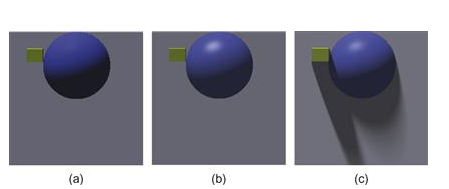
\includegraphics[width=\linewidth]{shading.png}
        \caption{Three types of shading}
    \end{figure}
    \begin{figure}[H]
        \centering
        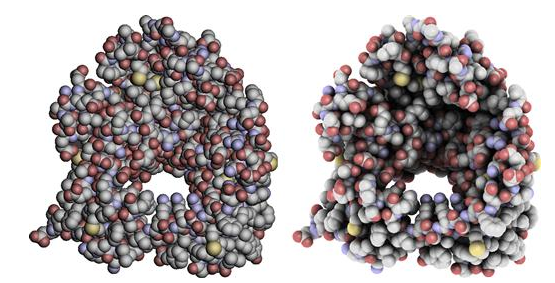
\includegraphics[width=\linewidth]{occlusion.png}
        \caption{Occlusion in a molecule visualization}
    \end{figure}

    \begin{figure}[H]
        \centering
        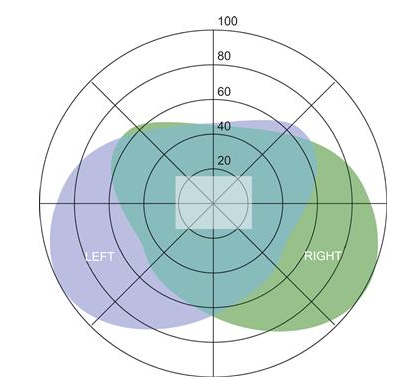
\includegraphics[width=0.6\linewidth]{visual_field.png}
        \caption{Visual field. Center square is a typical monitor}
    \end{figure}
\end{multicols}\end{mdframed}


\begin{mdframed}\begin{multicols}{2}
\subsection{The Eye}
    We do not see what is on the retina. The locus of conscious
    perception is higher up, with details lost.
\begin{compactdesc}
\item[Visual angle] angle subtended by an object at the eye of an observer.
    When 57cm away, 1cm is about 1 degree. Good apprx. for computer monitors.
\item[Lens] 59 diopters. Becomes less flexible with age. Lose about 2
    diopters per decade.
\item[Depth of Focus] At 50cm 43cm are near and 60cm are far. At 3m, 1.5m is
    near and $\infty$m is ``far''.
\item[Augmented reality] Superimpose visual imagery on the real world.
    Perspective is easy, eye position is difficult as is the design of
    optic systems to make light, undistorted and portable systems.
\item[Virtual reality] optical blur and optical distance must be simulated
    to accurately show depth. Eye tracker to determine the user's focus.
\item[Chromatic aberation] our eye is uncorrected for this. Blue on black is
    nearly indistinguishable. Can cause strong depth effects! Red on black
    seems nearer than blue on black for most people, though effect can be
    reversed.
\item[Retina] has two photoreceptor cells: rods (100 million) for low-light
    conditions, they are usually too stimulated to provide help and cones which
    are sensitive under normal levels (6 million).
\item[Fovea] center of the retina, densely packed only with cones. 2-degree
    field, best in the central $\frac{1}{2}$ degree.
\item[Simple acuities]:
    \begin{compactdesc}
    \item[Point (a)] acuity (1 minute of arc)
    \item[Grating (b)] acuity, bars (1 to 2 minutes of arc)
    \item[Letter (c)] acuity (5 minutes of arc). 20/20 vision means a 5 minute
        letter can be resolved 90\% of the time.
    \item[Stereo (d)] acuity, for depth (10 seconds of arc)
    \item[Vernier (e)] acuity, ability to see if two line segments are colinear
        (10 seconds of arc)
    \end{compactdesc}

\item[Binocular abilities] to perceive acuities improves by 7\% and
    contrast sensitivity increased by $\sqrt 2$.
\item[Acuity distribution] Only $\frac{1}{10}$ of detail 10 degrees from the
    fovea. Inverse square law.
\end{compactdesc}
\end{multicols}
\end{mdframed}


\begin{mdframed}\begin{multicols}{3}
    \begin{figure}[H]
        \centering
        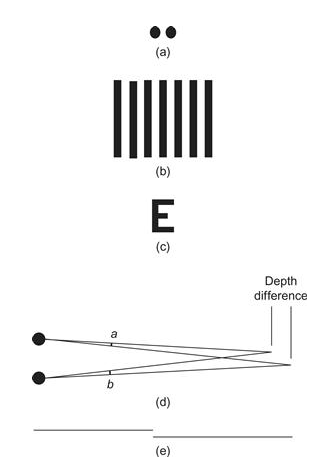
\includegraphics[width=0.7\linewidth]{acuities.png}
        \caption{Simple acuities}
    \end{figure}
    \begin{figure}[H]
        \centering
        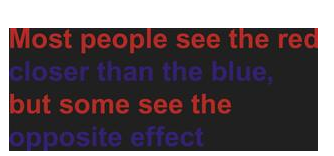
\includegraphics[width=\linewidth]{red_or_blue_near.png}
        \caption{Chromatic aberration}
    \end{figure}
    \begin{figure}[H]
        \centering
        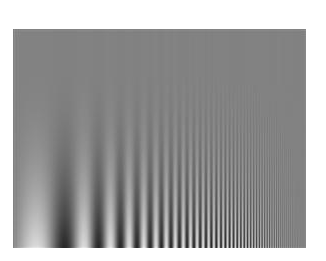
\includegraphics[width=\linewidth]{grating_gradient.png}
        \caption{Gradient along a grating pattern}
    \end{figure}

\end{multicols}\end{mdframed}




\begin{mdframed}
\begin{multicols}{2}
\begin{compactdesc}
\item[Axon] Thousands of photoreceptors (fewer in periphery) $\to$ ganglion
    cell, this is a type of neuron and it communicates using an axon. 3\% of
    the visual field receives half of the V1 neurons.
\item[Receptive field] area that feeds the retinal ganglion cells.
\item[Brain pixels] ganglion cells are the best match. Not uniformly
    distributed.
\item[Optimal screen]
    There are formulas for calculating efficiency of a
    screen. Though a typical monitor is only 5\% to 10\% of our visual field,
    it stimulates 50\% of our brain pixels. Small, high resolution with an
    interactive program beats low resolution and immersively large.
\item[Parafovea] best for pattern perception, 6 degrees, centered on fovea.
\item[Spatial contrast sensitivity] Most sensitive to dark bars on
    grey background at 2 to 3 cycles per degree. At age 80, less sensitive to
    $>1$ degree.
\item[Temporal contrast sensitivity] interdependent on spatial. Flicker. Most
    sensitive between 2 to 10 Hz.
\item[Visual stress] striped patterns of 3 cycles per degree, flicker at 20 Hz
    are the most likely culprits.
\item[Pattern-induced epilepsy] Avoid high contrast grating patterns or
    anything flickering at rates between 5 to 50 Hz.
\end{compactdesc}
\end{multicols}\end{mdframed}








\begin{mdframed}\begin{multicols}{2}
\subsection{The Optimal Display}
\begin{compactdesc}
\item[Dimensions] 4000 by 4000 pixels should be adequate. Printers use 1200
    dpi, this is to correct for the following two technical and one perception
    problem.
\item[Aliasing] mapping fine patterns to a pixel array causes errors. Our
    vernier acuity makes use sensitive to these problems. Fixed by computing
    a type of average of the input data, ``anti-aliasing. ''
\item[Number of dots] the 1200 dpi in a black and white printer are needed to
    print shades of gray. Aliasing effects are corrected by adding randomness
     to the dot position, instead of printing in square patches.
\item[Superacuities and displays] antialiasing enhances vernier acuity;
    even if the lines are subpixel size.
\item[Temporal requirements] our resolution limit is 50 Hz. Artifacts can be
    seen if the object moves too fast. Motion blur can fix.
\end{compactdesc}
\end{multicols}\end{mdframed}


